\documentclass[12pt,article,a4paper,english,brazil]{abntex2}

\usepackage[brazil]{babel}
\usepackage[left=3.0cm,top=3.0cm,right=2.0cm,bottom=2.0cm]{geometry}
\usepackage{indentfirst}
\usepackage{graphicx}
\usepackage{xcolor}
\usepackage{microtype} 			% para melhorias de justificação
\usepackage[alf]{abntex2cite}	% CITAÇÕES PADRÃO ABNT
\usepackage{fontspec}
\setmainfont{Arial}

% O tamanho do parágrafo(recuo) é dado por:
\setlength{\parindent}{1.25cm}
\linespread{1.5}

\selectlanguage{brazil}

\makeatletter
\hypersetup{
      pdftitle={\@title}, 
		  pdfauthor={\@author},
	    pdfcreator={Hugo Soares},
      pdfkeywords={VLC}{Visible Light Communication}{Raspberripy}{Dom Helder},
  		colorlinks=true,
    	citecolor=black,
      linkcolor=black,
      urlcolor=blue,
	    bookmarksdepth=4
}

\addto\captionsbrazil{
%% ajusta nomes padroes do babel
\renewcommand{\bibname}{Referências}
\renewcommand{\indexname}{Índice}
\renewcommand{\listfigurename}{Lista de ilustrações}
\renewcommand{\listtablename}{Lista de tabelas}
%% ajusta nomes usados com a macro \autoref
\renewcommand{\pageautorefname}{página}
\renewcommand{\sectionautorefname}{seção}
\renewcommand{\subsectionautorefname}{subseção}
\renewcommand{\paragraphautorefname}{parágrafo}
\renewcommand{\subsubsectionautorefname}{subseção}
}

\data{2023}

\begin{document}
  
  \titulo{VLC(Visible Light Communication)}
  \autor{Hugo Oliveira Soares}
  \local{Belo Horizonte}
  \instituicao{Dom Helder Escola Superior}
  \orientador{Prof. Marden Cicarelli Pinheiro}
  \coorientador{Prof. Ricardo Luiz de Freitas}
  \preambulo{
    Projeto de Pesquisa apresentado à Dom Helder Escola Superior como requisito parcial para obtenção do título de Cientista da Computação.
    \newline 
    \newline
    Orientador de conteúdo: \imprimirorientador
    \newline
    \newline
    Orientador de metodologia: \imprimircoorientador
  }

  % PARTE PRÉ-TEXTUAL
  \include{capa} 
  \makeatletter
\renewcommand{\folhaderostocontent}{
  \begin{center}

    \vspace*{\fill}
    \vspace*{\fill}
    \begin{center}
      \ABNTEXchapterfont\bfseries\Large\imprimirtitulo
    \end{center}

    \vspace*{\fill}

    \abntex@ifnotempty{\imprimirpreambulo}{
      \hspace{.45\textwidth}
      \begin{minipage}{.5\textwidth}
        \SingleSpacing
          \ABNTEXfontereduzida
          \imprimirpreambulo
      \end{minipage}
      \vspace*{\fill}
    }


    \vspace*{\fill}

    \imprimirlocal
    \par
    \imprimirdata
    \vspace*{1cm}

    \end{center}
}
\makeatother

  \imprimircapa
  \imprimirfolhaderosto

  \listoffigures
  \begin{siglas}
  \item[VLC]  Visible Ligth Communication
  \item[RF]   Radiofrequência
\end{siglas}

  \newpage
  \tableofcontents %SUMARIO

  %% CAPITULOS
  \section{Introdução}

Atualmente possuímos redes sem fios em praticamente qualquer lugar, porém ainda há locais onde as transmissões usando ondas eletromagnéticas não são desejáveis. Como por exemplo em voos e hospitais, devido às possíveis interferências nos aparelhos do hospital ou na comunicação do avião com a torre. Outro local onde a radiofrequência não é muito utilizada é debaixo d'água, devido a alta condutividade elétrica da água, assim prejudicando a transmissão.

Uma forma para resolver os problemas citados acima seria uma nova forma de transmissão de dados e um forte candidato para isso é o VLC (Visible Ligth Communication). Que é um sistema de comunicação por luz visível, ou seja, modula a informação e a transmite informações na faixa do espectro que varia entre 390 nm a 700nm.

\begin{figure}[h]
  \centering
  \caption{Espectro eletromagnético}
  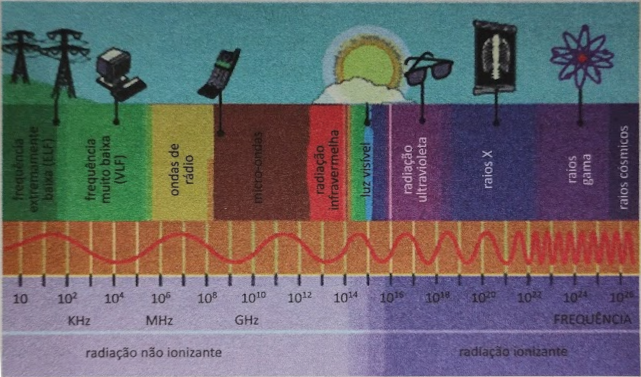
\includegraphics[width=0.8\textwidth]{images/espectro_eletromagnetico.png}
  
  \legend{Fonte: \citeonline[p. 9]{ondas}}
\end{figure}


Um dos pontos que fazem o VLC ser uma solução é o baixo custo, pois utiliza leds para a comunicação. Tal componente tem alta durabilidade e baixo consumo de energia, além de ser possível aproveitar a luz na iluminação no caso de um ambiente fechado, já que a transmissão é muito veloz a variação da iluminação é imperceptível ao olho humano.

  % \section{hipóteses} 
Este texto já se encontra no padrão de espaçamento correto. Ao elaborar o seu conteúdo, verificar se o espaçamento entre linhas é de 1,5 e se há uma linha livre entre parágrafos com espaçamento 0 pt antes e depois. 

Hipótese é sinônimo de suposição e premissas. É a tese a ser defendida no trabalho e, por ter tal característica de “possibilidade” de resposta, no final da pesquisa ela poder ser confirmada ou refutada.  

É destinada a explicar provisoriamente um problema até que os fatos venham a contradizê-la ou confirmá-la. É uma proposição testável que pode vir a ser a solução do problema.\newline
Portanto, de forma muito simples, é a “resposta provisória” para o problema de pesquisa formulado em relação ao tema (apresentado no tópico anterior).   

  \section{Objetivos}
\subsection{Objetivo geral}

Este texto já se encontra no padrão de espaçamento correto. Ao elaborar o seu conteúdo, verificar se o espaçamento entre linhas é de 1,5 e se há uma linha livre entre parágrafos com espaçamento 0 pt antes e depois. 

Indique de forma genérica qual objetivo deve ser alcançado. Está ligado a uma visão global e abrangente do tema. Relaciona-se com o conteúdo geral a ser apresentado como resultado, do problema de pesquisa.   

\subsection{Objetivos específicos}

Este texto já se encontra no padrão de espaçamento correto. Ao elaborar o seu conteúdo, verificar se o espaçamento entre linhas é de 1,5 e se há uma linha livre entre parágrafos com espaçamento 0 pt antes e depois. 

Têm função intermediária e instrumental, aplicado a situações particulares. São desdobramentos do objetivo geral, como as etapas a serem cumpridas para atingir o mesmo. Apresentam caráter mais concreto. Para construir este tópico, responda: “para quem fazer”? 

Não é uma regra, mas em geral são os capítulos e seus tópicos na composição do trabalho. 

Lembre-se:  
\begin{itemize}

 \item Usar verbos no infinitivo, tais como: verificar, avaliar, identificar, explicar, etc. 

 \item Servem para responder à pergunta: “O QUÊ?” 

 \item Objetivo é sinônimo de meta, fim. Indica o que o pesquisador quer atingir com o trabalho de pesquisa (o que você quer fazer, que metas você quer alcançar).  

 \item Devem ser apresentados em tópicos 
\end{itemize}

\cite{OpenVLC}

  \section{Justificativa}

Este texto já se encontra no padrão de espaçamento correto. Ao elaborar o seu conteúdo, verificar se o espaçamento entre linhas é de 1,5 e se há uma linha livre entre parágrafos com espaçamento 0 pt antes e depois. 
\cite{conceiccao2015comunicaccao}

\textit
A justificativa responde à pergunta “POR QUÊ?” 

Como o próprio nome indica, é o convencimento de que o trabalho de pesquisa deve ser efetivado.  

Apresente a relevância técnica, científica e socialmente sua proposta. Explicite argumentos que indiquem que sua pesquisa é significativa, importante ou relevante.  

Para ajudar, tente pensar nos três itens que não podem deixar de ser observados na justificativa. 

a) IMPORTÂNCIA: Que revela o porquê de se estudar tal tema. Por que o estudo desse tema é importante para a área em questão (Inteligência Artificial, por exemplo) e importante para você (pesquisador)? Aqui se concentra a chamada justificativa científica.  

b) VIABILIDADE: Quais são as possibilidades de se realizar esta pesquisa? Este aspecto está relacionado às possibilidades materiais da pesquisa: fontes de consulta disponíveis, etc. 

c) OPORTUNIDADE: Por que esta pesquisa é oportuna neste momento? Ela está de acordo com os interesses da atualidade? Aqui se concentra a chamada justificativa social-científica, que demonstra contribuição de seu conhecimento para a sociedade. 

Portanto, podem ser justificativas de ORDEM PESSOAL (relacionadas aos interesses dos pesquisadores, experiência ou possibilidade de atuação na área selecionada), de ORDEM TÉCNICA (acesso ao material e fontes de pesquisa, como livros, estatísticas, informações sobre a empresa) e ORDEM CIENTÍFICA (com a contribuição para a área do conhecimento, por ser um tema novo ou já existente e não satisfatoriamente respondido na área acadêmica, com espaço para novos debates). 

  % \include{capitulos/referencialTeorico}
  % \include{capitulos/metodologia}

  \bibliography{referencias}

\end{document}
